
\documentclass{standalone}
\usepackage{xcolor}
\usepackage{pgfplots}
\pgfplotsset{compat=1.18}

\begin{document}

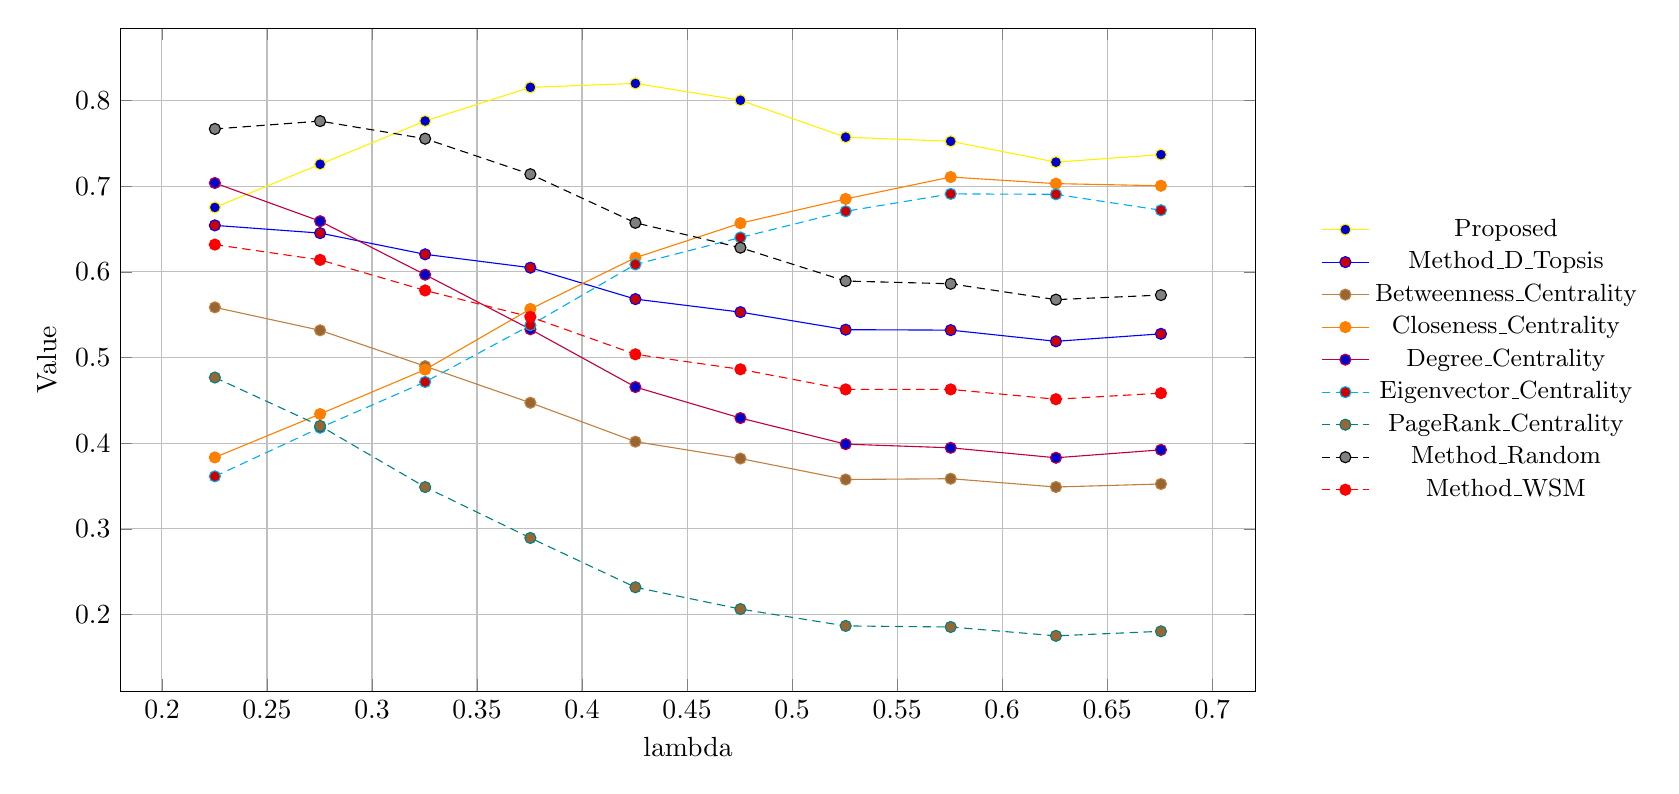
\begin{tikzpicture}
\begin{axis}[
    width=16cm,
    height=10cm,
    xlabel={lambda},
    ylabel={Value},
    grid=major,
    legend style={
        at={(1.05,0.5)},
        anchor=west,
        font=\small,
        draw=none,
        cells={align=left},
    },
]
% Proposed
\addplot+[color=yellow, mark=*] coordinates {
(0.2252,0.6751640576421526) (0.2753,0.7256285609741236) (0.3253,0.7761163610966424) (0.3754,0.8154053074148816) (0.4254,0.8199217960065078) (0.4754,0.800276066876158) (0.5255,0.7572005993165228) (0.5755,0.752410021094644) (0.6256,0.7280531060306039) (0.6756,0.7368451446574718) };
\addlegendentry{Proposed}

% Method\_D\_Topsis
\addplot+[color=blue, mark=*] coordinates {
(0.2252,0.6542408954417765) (0.2753,0.6452201512353128) (0.3253,0.6204412639823436) (0.3754,0.604847210745588) (0.4254,0.5681576413173808) (0.4754,0.5529654401735385) (0.5255,0.5324789001212823) (0.5755,0.5319372753185435) (0.6256,0.5188924655831763) (0.6756,0.5276115625549375) };
\addlegendentry{Method\_D\_Topsis}

% Betweenness\_Centrality
\addplot+[color=brown, mark=*] coordinates {
(0.2252,0.5585328369499392) (0.2753,0.5317299567174766) (0.3253,0.4898323011079129) (0.3754,0.4471579852267162) (0.4254,0.4017622874122586) (0.4754,0.3820296850698262) (0.5255,0.3575478216418337) (0.5755,0.3584797283624016) (0.6256,0.3487833230799915) (0.6756,0.3523173961999013) };
\addlegendentry{Betweenness\_Centrality}

% Closeness\_Centrality
\addplot+[color=orange, mark=*] coordinates {
(0.2252,0.3833487810087244) (0.2753,0.4340031707568612) (0.3253,0.4858883104827247) (0.3754,0.5566067118949168) (0.4254,0.6164614398419589) (0.4754,0.6567635325089756) (0.5255,0.685103655738207) (0.5755,0.7106685383413258) (0.6256,0.7029703563536722) (0.6756,0.7005094791330894) };
\addlegendentry{Closeness\_Centrality}

% Degree\_Centrality
\addplot+[color=purple, mark=*] coordinates {
(0.2252,0.7037207007065506) (0.2753,0.659098723073716) (0.3253,0.5966477618644872) (0.3754,0.5329339368789596) (0.4254,0.4655052805488709) (0.4754,0.4292839825199682) (0.5255,0.3988380325373307) (0.5755,0.3945642835240934) (0.6256,0.3829222715006277) (0.6756,0.3921693406161655) };
\addlegendentry{Degree\_Centrality}

% Eigenvector\_Centrality
\addplot+[color=cyan, mark=*] coordinates {
(0.2252,0.3612100247207835) (0.2753,0.4180021120273026) (0.3253,0.4714507629790717) (0.3754,0.5376587892244636) (0.4254,0.6086524276620314) (0.4754,0.6401071474111449) (0.5255,0.6706787113164059) (0.5755,0.6909979774656075) (0.6256,0.6904820753447553) (0.6756,0.6719213592538721) };
\addlegendentry{Eigenvector\_Centrality}

% PageRank\_Centrality
\addplot+[color=teal, mark=*] coordinates {
(0.2252,0.4766298377497861) (0.2753,0.4201552190327844) (0.3253,0.34870322305566) (0.3754,0.2893139547208012) (0.4254,0.2317345830400997) (0.4754,0.206306361826683) (0.5255,0.1866034618747558) (0.5755,0.1853709457910453) (0.6256,0.1750199252928288) (0.6756,0.1803193907350797) };
\addlegendentry{PageRank\_Centrality}

% Method\_Random
\addplot+[color=black, mark=*] coordinates {
(0.2252,0.7668182658917511) (0.2753,0.7759681254555331) (0.3253,0.7554468768973347) (0.3754,0.7139786979879557) (0.4254,0.6572346824236557) (0.4754,0.6282040221083809) (0.5255,0.5892554966778106) (0.5755,0.5860659692803399) (0.6256,0.5675311682166198) (0.6756,0.572880232812798) };
\addlegendentry{Method\_Random}

% Method\_WSM
\addplot+[color=red, mark=*] coordinates {
(0.2252,0.6317791740189266) (0.2753,0.6139584002735365) (0.3253,0.5782597798758372) (0.3754,0.5473820808322821) (0.4254,0.5037085841049337) (0.4754,0.4861957897158632) (0.5255,0.4627272204627362) (0.5755,0.4627473923437829) (0.6256,0.4512829887965646) (0.6756,0.4583619288696581) };
\addlegendentry{Method\_WSM}


\end{axis}
\end{tikzpicture}

\end{document}
